%TEX root = ../dissertation.tex

\chapter{Solution}
\label{chapter:solution}
% Overview about the solution
% Types of users
% For each one, who he is, what he does...
% What was implemented for each one
The main goal of our solution is to assist
the development process of proximity-based mobile applications.
Before starting the description of our solution we need to take a look at three kinds of users that will be part of it:
\begin{description}
  \item[End users] are anyone with a mobile device that installs an app to scan for nearby Smart Places and interact with tags;
  \item[Owners] are responsible for managing a given place that they want to turn into a Smart Place;
  \item[Developers] develop the code for the Smart Places.
\end{description}

The Smart Places solution has a component that targets each one of the presented type of user.
There is a mobile app to allow anyone with a mobile device to use the services provided by nearby Smart Places.
Owners have a mobile app that allows them to turn the places they manage into Smart Places.
To develop these services our solution offers an \gls{API} that developers can integrate in their web applications to make them react to the presence of the user.

% What comes next
Next, we present related work about existing proximity-based applications and tools.
Section \ref{sec:solution_solution_overview} introduces the main components of the solution and how they relate with each other.
The Android apps are described in sections \ref{sec:solution_mobile_app_for_end_users} and \ref{sec:solution_mobile_app_for_owners}, respectively.
Then, we present the \gls{API} for developers in section \ref{sec:solution_developers_api}, from its installation to its usage.
In section \ref{sec:solution_examples}, we describe two examples of Smart Places, the Smart Restaurant and the Smart Museum, including their main features and how they contributed to the development of our Developers \gls{API}.
Finally, in section \ref{sec:solution_summary} there is a summary of the important aspects of our solution.

\section{Related Work}
\label{sec:background_related_work}
% Related work...
Here we discuss related work in order to have a good insight about the possibilities and existing solutions for the problem we are trying to solve.

\subsection{Proximity-based Apps}
\label{sub:background_ble_beacons_applications}
% Why
% For each one: What, Pros, Cons
\gls{BLE} Beacons were
used to develop our solution, based on the concept of Smart Places.
Some applications where this technology is used
are presented here to
get good insights about the potential use cases of this
technology and the apps developed using it.
\begin{description}
  \item[BlueSentinel\cite{Conte2014}]
  is a
  occupancy detection system for smart buildings
  that uses \gls{BLE} Beacons to detect the presence of
  people. The concept of a smart building
  is similar to Smart Place
  due to the existence of sensors and actuators.
  It is focused on the power efficiency of the
  building.
  The idea is to optimize energy
  consumption according to people's presence.
  For instance, if there are no people in a given room
  the heating system can be turned off.
  In this solution the users have to install
  an app that will get the beacons' signal and
  send data to a server, which will process it
  and send requests to actuators in order to
  perform actions to optimize the
  building's power efficiency.
  Unfortunately, there is a limitation
  of iBeacon protocol implementation
  in iOS.
  Beacons can be received by the apps
  only when these are active. When the apps are in
  background they are waken up only to handle
  enter/exit region events. To circumvent this
  limitation the authors developed custom
  beacons which advertise more than one region
  in a cyclic sequence. These custom beacons
  were created using an
  Arduino\footnote{http://www.arduino.cc/}
  and a Bluetooth \gls{USB} dongle.
  Since this solution is a native app
  users have to install it in order
  to make the smart building work to
  optimize power efficiency.
  Once the user starts the app, he/she does not
  need to interact with it anymore since it
  will run in background.
  \item[BlueView\cite{Chen2013}]
  is a system to help
  visually impaired people to perceive some points of interest.
  This solution has two main components: The viewer device
  and the \glspl{BP}. The first one is a mobile phone,
  carried by the user, which is bluetooth enabled.
  The \glspl{BP} are just bluetooth tags instead of
  \gls{BLE} Beacons. The name of a point of interest is associated with the
  \gls{MAC} address of the tag which it is associated to.
  The steps involved in using the system are the
  following: first, the viewer device will scan
  for nearby \glspl{BP}; then, a list of the names of
  \glspl{BP} is created. This list is refreshed anytime a new
  \gls{BP} is detected and the user is informed through auditory feedback.
  The second step consists of the user using
  the viewer's device establishing a connection with a \gls{BP}
  attached to an object. Finally, using audio prompt, the \gls{BP}
  will assist the user in locating the object.
  Despite of this solution being a mobile app, installed
  in the viewer's device the authors do not have in
  consideration the typical concerns of any mobile app,
  such as the energy consumption.
  The authors tested the application, in 2013,
  using Nokia N70 as the viewer device.
  This solution could be implemented using \gls{BLE} Beacons
  and the viewer device could be any Android or iOS smartphone.
  \item[ContextCapture\cite{Antila2011}]
  uses context-based information to allow users to
  add more information to their status updates
  in the main social networks, such as
  Facebook\footnote{http://www.facebook.com} and
  Twitter\footnote{http://twitter.com}.
  This work had two main goals: first, demonstrate technical
  aspects of collaborative context such as,
  how to get contextual information from
  surrounding devices and how they can be used
  as a source of contextual information;
  second, test and analyze the user experience of
  context-aware systems.
  The user can decide the abstraction level (coordinates,
  address or semantic label).
  The authors implemented a mobile app and a
  server integrated with Facebook and Twitter.
  Context information comes from the smartphone itself,
  from its sensors and from the nearby devices through
  Bluetooth.
  Devices can be other smartphones or \gls{BLE} Beacons which
  are used for indoor location.
  Similar to \cite{BenAbdesslem2014}, devices communicate
  with each other as a network.
  Using this solution, the user can create status updates
  in the mentioned social networks in the format shown in Listing~\ref{lst:context_capture_status_update}:
  \begin{listing}[H]
      [User-defined message]

      Sent from [Location] while [Activity]

      [Description] [Topic] and [Applications Activity] with
      [Friends].
    \caption[ContextCapture update format]{Format of status updates in ContextCapture}
    \label{lst:context_capture_status_update}
  \end{listing}
\end{description}

\subsection{Context-aware applications}
\label{sub:frameworks_context_aware}
In this section we describe related work about the
development of mobile native and web
context-aware applications.
Since we have created a framework to develop
proximity-based services, the state
of the art of existing frameworks that deliver
context information to the apps will be presented.
\begin{description}
  \item[Frameworks for developing distributed
  location-based applications:]
  There are frameworks to develop location-based
  applications.
  In the work presented in Krevl et al.\cite{Krevl2006},
  a framework
  was developed to allow developers to build
  location-based apps. Location information can come
  from any source, such as \gls{GPS}, Bluetooth and \gls{WiFi} receivers.
  The authors discuss some benefits and limitations
  of several technologies for getting the
  user's location.
  In terms of architecture, the main components
  are:
  \begin{itemize}
  \item
  Devices that are used to get location data, such as
  the ones already mentioned;
  \item The users' mobile devices;
  \item The Database Server, which is where the mapping
  between geographical coordinates and location
  information is stored;
  \item And, the Application Server, which provides web services for
  mobile clients.
  This server also communicates
  with the Database Server.
  \end{itemize}
  The mobile device gets geographical coordinates
  from any source and send that data in a
  \gls{SOAP}\cite{Seely:2001:SCP:560836} message,
  to the appropriate web service in the Application
  Server. This server communicates with the Database Server
  to query the database, which sends back a response with
  location information, if there is any, for that
  particular group of geographical coordinates.
  The authors did not evaluate the system.
  \item[Dynamix\cite{dynamix}]
  is a framework to develop
  mobile native and web apps that allows them to receive
  context information for instance, position and device's
  orientation. This framework has plugins that get
  one or more sensor's raw data and turn that into event
  objects that contain more high-level information.
  This framework supports many kinds of context information
  and it is possible to develop more plugins to allow the
  apps to generate additional events that are not
  already supported.
\end{description}

\subsection{Discussion}
\label{sub:solution_related_work_discussion}
In order to get a good insight about the potential of proximity-based services, we analyzed three applications.
The BlueSentinel is a system that uses \gls{BLE} beacons to detect the presence of people in a building. It tries to optimize energy consumption based on people's presence.
Another one, BlueView, is a system to help visually impaired people to be aware of some points of interest.
The third is the ContextCapture that allows users to create status updates on social networks using context information.

We introduced a framework to develop distributed location-based applications and a more generic one that targets the development of context-aware applications.
For each one, we described the idea, its main components, in order to get an overview about their limitations, which we try to circumvent in our solution.
However, most of them only helps developers to write native apps, that is, apps written for a specific platform that will run only on it.
This leads to a situation where the user needs to install one app, in his/her mobile device, for each proximity-based service he/she wants to use.
In order to circumvent this limitation, this solution allows developers
to use the same technologies that are used for any web application such as \gls{HTML}, \gls{CSS} and Javascript to build Smart Places allowing them run on a web browser that can be embedded in a mobile app. This way, users only need to install one app to discover and use proximity-based services following the Smart Places approach.

The framework described in Krevl et al.\cite{Krevl2006} offers abstractions for the location information sources.
Geographical coordinates can
come from any source.
It is a good approach for
mobile native apps but it does not support web apps.
The authors do not take into consideration
constraints in terms of resources, such as
lack of Internet connection and battery.
Since most users have limited data plans for
their smartphones and \gls{SOAP} messages can
grow in size due to its \gls{XML} format,
a more efficient message encoding could be used
instead, for instance \gls{REST} using \gls{JSON}.

To achieve our goal, our framework could be just a
plugin for Dynamix. The plugin would
need to get the beacon's raw data and
turn that into a more high-level information
using a backend. In this framework,
the user needs to install an app that manages the service
that runs in background and needs to define some
security policies such as which information the app can have access to or which sensors it can use.
This could mean a big overhead since we are more focused on developing proximity-based applications that do not require such complex security policies because in this kind of applications, there is only need to access the device's sensors that could provide positioning data to the applications.

\section{Solution Overview}
\label{sec:solution_solution_overview}
% Introduce solution
% Smartphone
% App for owners
% App for users
% API for developers
% Beacons (Tags)
% Backend
The Smart Places solution developed in this work is composed by several components, as shown in Figure~\ref{fig:solution_overview}:
\begin{description}
  \item[Beacons]
  are the small devices that will act as tags, according to our definition of a Smart Place;
  \item[Backend]
  is where all the data about Smart Places is stored, that is, that are available and the ones tht the owner has configured, information about each beacon, etc;
  \item[End Users Mobile App]
  is an Android mobile app that allows users with a mobile device \gls{BLE} enabled to have access to nearby Smart Places and to detect the beacons that belong to those Smart Places;
  \item[Owners Mobile App] is another Android mobile app that owners use to select which Smart Places they want to configure. It also allows to configure each individual beacon that belongs to a given Smart Place;
  \item[Developers \gls{API}] provides the necessary methods that developers can use to create their proximity-based services, based on the concept of a Smart Place.
\end{description}
Each mentioned component is described, in further detail, in the next sections.

\begin{figure}[!ht]
  \centering
    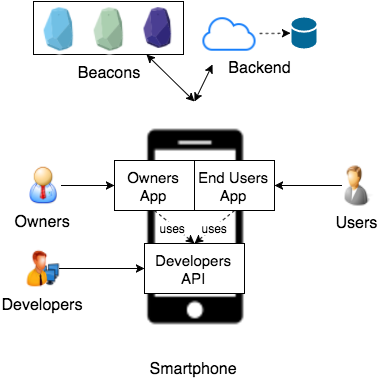
\includegraphics[width=0.7\textwidth, keepaspectratio]{images/smart_places_solution_overview}
    \caption[Solution Overview]{Overview with the main components of Smart Places solution}
    \label{fig:solution_overview}
\end{figure}

\section{Mobile App for End Users}
\label{sec:solution_mobile_app_for_end_users}
% Who are end users
% What are the main features of the app
% Workflow (whith some screenshots)
Anyone that has a mobile device, such as a smartphone, can use the services provided by any Smart Place.
In our solution, there is an Android app distinct from the one described in section \ref{sec:solution_mobile_app_for_owners}, that notifies the user when he is nearby any Smart Place.
When the mobile device approaches any Smart Place the app notifies the user that he is near a Smart Place.
When the user touches these notifications the app shows an embedded web browser that contains a web page that can react to nearby objects, that is, beacons with meaning to the application.

After installing the app, the first time the user opens it, the app ask the user to turn on the device's bluetooth, as shown in Figure~\ref{fig:screenshot_clientapp_entry}.
\begin{figure}[!ht]
  \centering
    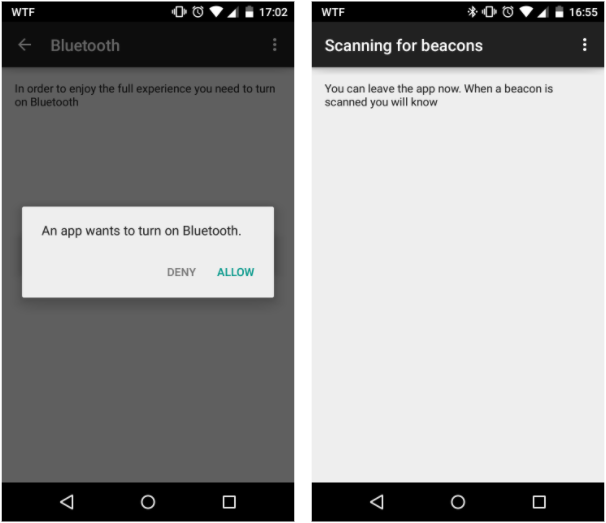
\includegraphics[width=0.7\textwidth, keepaspectratio]{images/screenshots/clientapp_entry}
    \caption[Users mobile app]{First interaction with the user}
    \label{fig:screenshot_clientapp_entry}
\end{figure}
This app will scan for nearby beacons periodically.
Each time a beacon is scanned, the app shows a notification associated to a Smart Place.
If the scanning period is small, the app can constantly notify the user. Otherwise, if this period is big the user will receive less notifications.
This period also has an impact on battery consumption.
The more times the app scans for nearby beacons the more battery is drained.
According to his/her preference, our app allows the user to change the scan periods in background and foreground modes.

\section{Mobile App for Owners}
\label{sec:solution_mobile_app_for_owners}
% Who are the owners
% What are the main features of the app
% Workflow (with some screenshots)
The Smart Place owners manage one or more places where they want to provide a service to visitors in their mobile devices.
In order to make owners be able to offer this kind of services, an Android app designed for them is offered by this solution.
This app offers the folllowing features:
\begin{itemize}
  \item Get a list of all available Smart Places;
  \item Configure an instance of a given Smart Place;
  \item Delete an existing configuration of a given Smart Place;
  \item Update an instance of a given Smart Place.
\end{itemize}

In order to configure a Smart Place first, owners need to tag physical objects.
They need to deploy beacons in the right places.
Then, they use the mobile app to create an instance of a Smart Place following the steps shown in Figure~\ref{fig:screenshot_ownersapp}:
\begin{itemize}
  \item First, the app asks owners to log in.
  The app only allows log in using user's Facebook account.
  Parse \gls{BaaS} already provides integration with social networks.
  We did not need to ask for an username and password.
  \item The app shows a list of all available Smart Places that the owner can configure.
  For instance, the Smart Restaurant and Smart Museum examples described in section \ref{sec:solution_examples} are examples of Smart Places that can appear in this list;
  \item Then, the owner selects one and he can see a text explaining what that Smart Place is about;
  \item Finally, the owner just needs to type a title and a message, that will appear in the users' mobile devices notifications when they are nearby
\end{itemize}

After creating an instance of a Smart Place the owner needs to configure tags, that is, associate information to the previously deployed beacons.
This information will depend on the Smart Place.
Figure~\ref{fig:screenshot_ownersapp_configure} shows the needed steps to configure tags in an instance of a given Smart Place.
First, the owner selects the instance from the list of ones that he has created.
Then, he has access to an interface where he can manage the existing tags of that Smart Place instance.
Each Smart Place has its own management interface.
Developers are responsible for creating these interfaces, using the developers \gls{API}, introduced in section \ref{sec:solution_developers_api}.

\begin{figure}[!ht]
  \centering
    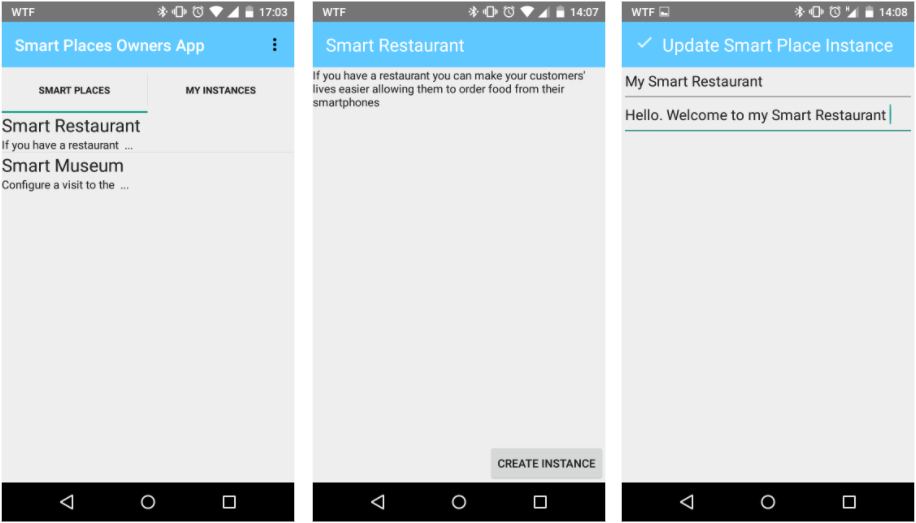
\includegraphics[width=1\textwidth, keepaspectratio]{images/screenshots/ownersapp}
    \caption[Create a Smart Place Instance]{From left to right, the steps to create an instance of a given Smart Place}
    \label{fig:screenshot_ownersapp}
\end{figure}

\begin{figure}[!ht]
  \centering
    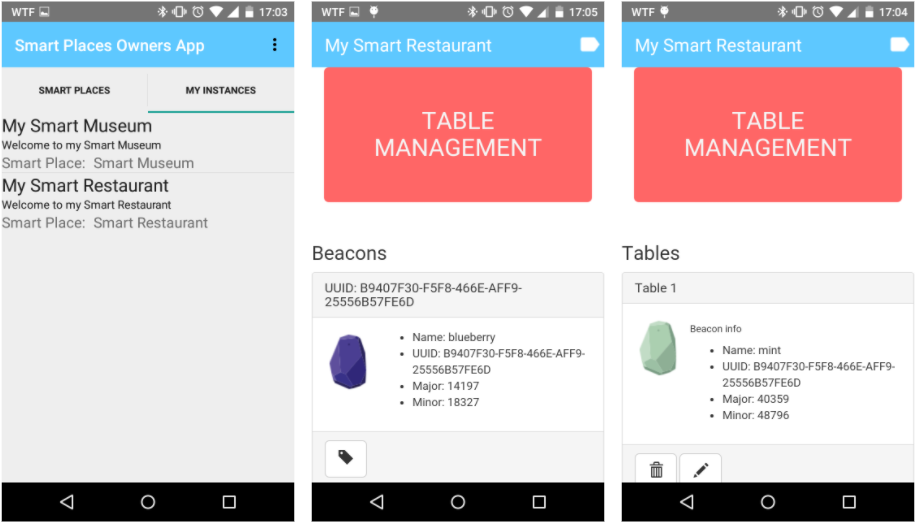
\includegraphics[width=1\textwidth, keepaspectratio]{images/screenshots/ownersapp_configure}
    \caption[Configure a Smart Place Instance]{From left to right, the steps to configure an instance of a given Smart Place}
    \label{fig:screenshot_ownersapp_configure}
\end{figure}

\section{Developers API}
\label{sec:solution_developers_api}
% Why javascript api
% Who
% How to use it (with some code snippets)
Owners configure the data of a Smart Place and end users can interact with objects nearby.
But, who will add behavior to these Smart Places?
Our solution offers a way for developers to create their Smart Places.
Also, we want to avoid the user having to install one mobile app for each Smart Place.
The app for end users has an embedded web browser, so they can use any Smart Place as they would use any web application without the need to install one more mobile app.
That is why a Javascript library is part of our solution.
This way, an existing web application can use this library and make it react to nearby objects tagged with \gls{BLE} beacons.

The library was turned into an open-source project, hosted on a github repository\footnote{http://github.com/samfcmc/smartplaces-js} and it is available to install using bower\footnote{http://bower.io}, which is a tool to manage dependencies in web applications.
If a developer wants to install this library, he/she just needs to run a command, as shown in Listing~\ref{code:bower_install}

\begin{listing}[H]
  \begin{minted}[xleftmargin=.1\textwidth]{shell}
  bower install smartplaces-js --save
  \end{minted}
  \caption[Library installation using Bower]{Command to install smartplaces-js library using bower}
  \label{code:bower_install}
\end{listing}
Then, he/she just needs to include the library and use the available functions.
The library is event-based, that is, the mobile apps described in sections \ref{sec:solution_mobile_app_for_owners} and \ref{sec:solution_mobile_app_for_end_users} emit events to the library such as, a nearby beacon is detected, to the web application running inside a embedded web browser.
In this library, there is a global object, which is ``SmartPlaces'' with several methods.
All those methods need to receive a callback because because as already mentioned the library follows an event-based approach.
The reason why it is not synchronous is explained in chapter \ref{chapter:implementation}, section \ref{sec:implementation_smart_places}.
However, developers are also responsible for creating the interface to configure the Smart Place, that is, the steps that owners have to follow, as described in section \ref{sec:solution_mobile_app_for_owners} after they select the Smart Place they want.
In the part of the web app that will be accessed by owners, developers first need to initialize the library, as shown in Listing~\ref{code:smartplaces_initialization}.
\begin{listing}[H]
  \begin{minted}[xleftmargin=.1\textwidth]{javascript}
    SmartPlaces.onInit(function(smartPlaceInstance) {
      // Code after initialization of this Smart Place Instance
    });
  \end{minted}
  \caption[Javascript library initialization]{Javascript library initialization}
  \label{code:smartplaces_initialization}
\end{listing}

When the owner is using the app, described in section \ref{sec:solution_mobile_app_for_owners}, there is a button that when is touched the app scans for nearby beacons and sends an event to the javascript library.
Developers have to define the behaviour when this event is emitted, as shown in
Listing~\ref{code:smartplaces_on_beacons_scanned}.

\begin{listing}[H]
  \begin{minted}[xleftmargin=.1\textwidth]{javascript}
    SmartPlaces.onBeaconsScanned(function(beacons) {
      // Code to handle beacons that were scanned
    });
  \end{minted}
  \caption[Beacons scanned]{Defining a callback function when beacons are scanned by the mobile app for owners}
  \label{code:smartplaces_on_beacons_scanned}
\end{listing}

The argument named ``beacons'' in the callback function in \ref{code:smartplaces_on_beacons_scanned} is an array of \gls{JSON} objects, where each one has the following keys:
\begin{itemize}
  \item uuid: The \gls{UUID} of the beacon that was scanned;
  \item major: The major value, according to the ibeacon protocol;
  \item minor: The minor value, according to the ibeacon protocol.
\end{itemize}

However, there is more information about each beacon for instance, its name and its icon \gls{URL}.
To get this extra information, from a beacon \gls{JSON} object, there is a function, which usage is shown in Listing~\ref{code:smartplaces_get_beacon}, that makes a request to the backend in order to get all the information about the given beacon. This information includes a name and an \gls{URL} for an image that represents the beacon, besides the data already provided such as the \gls{UUID}, major and minor values.
Since this function makes a request to the backend, we need to pass as an argument an object with two keys:
\begin{itemize}
  \item success: Callback function when the request was successfully made and we got a response with an object that, besides the keys mentioned before, \gls{UUID}, major and minor, also got the name and icon which is an \gls{URL} that we can use to get the image of that particular beacon;
  \item error: Callback function, when the request returns an error.
\end{itemize}

\begin{listing}[H]
  \begin{minted}[xleftmargin=.1\textwidth]{javascript}
    SmartPlaces.getBeacon(beaconScanned, {
      success: function(beacon) {
        /*
        Code to handle when a beacon object was retrieved
         successfully from the backend
        */
      },
      error: function(error) {
        /*
        Code to handle when an error occurrs when trying
         to get a beacon object from the backend
        */
      }
    });
  \end{minted}
  \caption[Get beacon object]{Get beacon information from the backend}
  \label{code:smartplaces_get_beacon}
\end{listing}

After we got the beacon object with all the information, it is possible to associate a \gls{JSON} with any structure.
To do that, there is an ``associateTag'' function which usage is illustrated in Listing~\ref{code:smartplaces_associate_tag}.
We need to pass the beacon object, the object with the data that we want to associate with the beacon and another object with success and error keys, similar to what is shown in Listing~\ref{code:smartplaces_get_beacon}.

\begin{listing}[H]
  \begin{minted}[xleftmargin=.1\textwidth]{javascript}
    SmartPlaces.associateTag(beacon, data, {
      success: function(tag) {
        /*
        Code to handle when a tag is successfully
        associated to a beacon
        */
      },
      error: function(error) {
        /* Code to handle when an error occurrs trying
        to associate a tag to a beacon
        */
      }
    });
  \end{minted}
  \caption[Associate tag]{Associate a tag to a given beacon and provide custom data}
  \label{code:smartplaces_associate_tag}
\end{listing}

It is also possible to update an existing tag.
For that, developers can use the ``updateTag'' function.
Its usage is shown in Listing~\ref{code:smartplaces_update_tag}.
This function requires the existing tag object and an object with success and error keys similar to the other functions that make requests to the backend.
This function is similar to the previous one, shown in Listing~\ref{code:smartplaces_associate_tag} but instead of passing a beacon as an argument, we pass a tag object to update it with the data in the object provided as the second argument.

\begin{listing}[H]
  \begin{minted}[xleftmargin=.1\textwidth]{javascript}
    SmartPlaces.updateTag(tag, data, {
      success: function(updatedTag) {
        /*
        Code to handle when the given tag is successfully updated
        */
      },
      error: function(error) {
        /*
        Code to handle when an error occurrs when
        trying to update the given tag
        */
      }
    });
  \end{minted}
  \caption[Update an existing tag]{Update data of a given tag}
  \label{code:smartplaces_update_tag}
\end{listing}

The previously mentioned functions, are available in order to make developers able to create the interfaces for owners.
For the end users, the mobile app detects nearby tags and emit an event to the web application running inside the embedded web browser.
Developers need to define a callback function for this event.
To do that, the ``onTagFound'' can be used, as shown in Listing~\ref{code:smartplaces_tag_found}.
The tag object, which is the argument of this callback function, is the \gls{JSON} object created previously in the code illustrated in Listing~\ref{code:smartplaces_associate_tag}.

\begin{listing}[H]
  \begin{minted}[xleftmargin=.1\textwidth]{javascript}
    SmartPlaces.onTagFound(function(tag) {
      // Code to handle when the mobile app detects a tag
    });
  \end{minted}
  \caption[Defining a callback for when a tag is found]{Callback for when a nearby tag is found}
  \label{code:smartplaces_tag_found}
\end{listing}

\section{Examples}
\label{sec:solution_examples}
% Why
% Introduce each one
% Explain the main features
We have created two examples of Smart Places to see if our solution would work in practice.
% Created one example, extracted one API, applied to other example
First, we developed the Smart Restaurant.
While building this example, we wrote Javascript code to handle the events emitted by the mobile apps, described in sections \ref{sec:solution_mobile_app_for_owners} and \ref{sec:solution_mobile_app_for_end_users}.
From this code, it was possible to create a library that resulted in a complete independent project, from which, the examples depend on.
After building the first example, we developed another one which is the Smart Museum.
We defined the Javascript library as a dependency and observed that the same \gls{API} that fits the Smart Restaurant example, also was used in the other example.
Also, we avoided to develop the examples completely from the scratch.
Instead, we tried to integrate the \gls{JS} \gls{API}, described in section \ref{sec:solution_developers_api} with existing applications or \glspl{API}.

As already mentioned, two examples were created.
The first, described in section \ref{sub:solution_smart_restaurant}, is a Smart Place for restaurants to allow customers to place their orders without the need to wait.
The other one, is a proximity-based service for museums.
It allows users to have access to more information about an object that they are close to in a museum exhibition.
Its features are described in section \ref{sub:smart_museum}.

\subsection{Smart Restaurant}
\label{sub:solution_smart_restaurant}
The Smart Restaurant was the first app created to show the usage of the entire solution.
The main goal here is to allow restaurants' customers to place their orders, using their mobile devices, such as smartphones, without having to wait for an employee coming to them.
When customers arrive at this Smart Restaurant, a notification shows up in their devices with a message saying that they can place their orders using the mobile app.
Then, they touch the notification and a new \gls{UI} appears.
Now, they have access to the restaurant's menu where they can pick what they want and in the end, place their orders.
Figure~\ref{fig:smart_restaurant_app}, shows the steps that the customer follows to place an order using the mobile app. We can see from left to right that the app detects the table's number and after the sign in process several buttons appear, each one representing a family of products and there is a button in the bottom to see the complete order.
When the customer touches this button, there is a list of the complete order and a button to send the order.

Also, there is a backoffice, where employees and managers, have access to an \gls{UI} to manage the orders and the menu.
This backoffice was implemented in another master thesis\cite{SLOC}.
Our work here was to integrate our solution in this backoffice.
There was already an interface to place orders.
We changed this interface to use our Developers \gls{API}, described in section \ref{sec:solution_developers_api} to get the table's number.
We also added an option to the backoffice's \gls{UI} to manage the mapping between tables and beacons.
This integration shows the hability to use existing code, that is, our Smart Places solution can be integrated in existing applications.

\begin{figure}[!ht]
  \centering
    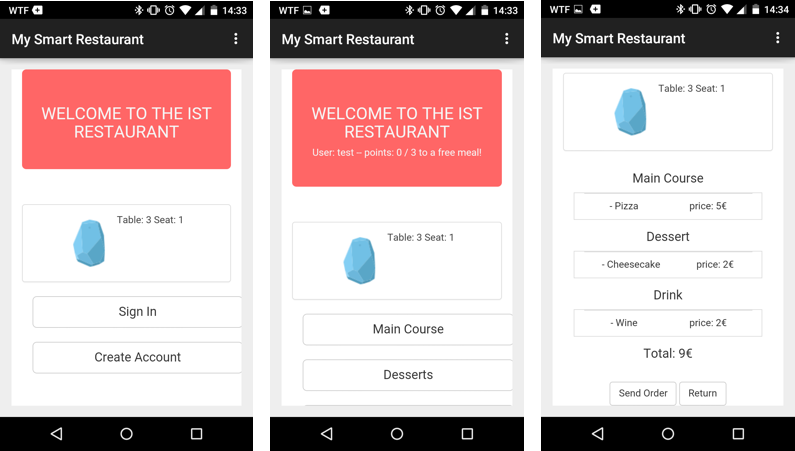
\includegraphics[width=0.8\textwidth, keepaspectratio]{images/screenshots/smart_restaurant_app}
    \caption[Smart Restaurant]{Steps to place an order in the Smart Restaurant app}
    \label{fig:smart_restaurant_app}
\end{figure}

\subsection{Smart Museum}
\label{sub:smart_museum}
The Smart Museum is another example of a Smart Place, that is, a proximity-based service developed using our solution.
The idea is to allow visitors of a museum to have access to information about a given object in a given exhibition using their mobile devices.
Visitors go to the museum and as they look at a given object they are notified, through the mobile app that they can get more information.
Then, when they touch in the notification, a screen appears with the information about that object that they are looking at.
Figure~\ref{fig:smart_museum_app} shows a screen, in the mobile device, after the museum's visitor has touched the notification.

\begin{figure}[!ht]
  \centering
    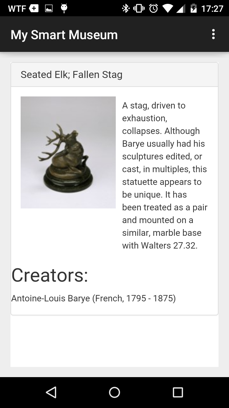
\includegraphics[width=0.4\textwidth, keepaspectratio]{images/screenshots/smart_museum_app}
    \caption[Smart Museum]{Smart Museum app showing information}
    \label{fig:smart_museum_app}
\end{figure}

Instead of creating a fake museum with mock data, we used real data from a real data source.
The idea was to try to emulate the real experience.
For that, we have used data from the Walters Art Museum\footnote{http://thewalters.org}, which is a public art museum, located in Mount Vernon-Belvedere, Baltimore, Maryland.
It was founded in 1934 and its collection includes more than 30 000 objects.
The way we got the data about the collections and objects is detailed in chapter \ref{chapter:implementation}, section \ref{sub:implementation_smart_museum}.

\section{Summary}
\label{sec:solution_summary}
% Related work
% -> Proximity-based apps (BlueSentinel and BlueVIew)
% -> Context-awareness
% -> Dynamix
In this chapter we reviewed related work and identified desirable features for better proximity based solutions.
% Targets owners, developers and end users
% Solution overview
% -> Components (Beacons, Backend, mobile apps, API)
We presented our Smart Places solution and its main components.
There are the beacons which act as tags in a Smart Place.
The Backend stores the data about each Smart Place and the tags.
Since our solution targets owners and end users, there is a mobile app for each one that offers features according to their needs.
Also, for developers, we introduced an \gls{API} that they can be used to create proximity-based services according to the definition of a Smart Place.

% Mobile App for End Users
% -> What it is
% -> Main features
The app for end users, anyone with a mobile device that can detect tags in a given Smart Place and then forward to specific functionalities.
The user needs to install the app and turn on the device's Bluetooth receiver.
Then, the app will scan for nearby beacons, in background.
When a Smart Place is found, the app notifies the user.
When the user touches a notification the app will perform a new scan but this time, to find tags that belong to that Smart Place.

% Mobile App for Owners
% -> What it is
% -> Main features
The mobile app for owners allows them to see a list of available smart places, configure an instance of a given Smart Place, delete an existing configuration or update an instance of a Smart Place they already have configured.
Owners deploy beacons in the right places and use the app to create an instance of a Smart Place and configure the tags according to what is requested by the Smart Place that he is configuring.

% Developers API
% Event based API
% -> How to install
% -> Overview of usage
Developers implement the custom behaviors of proximity-based services.
We created an \gls{API} for them to use to make the development of a Smart Place an easier process that without this \gls{API}.
Due to its asynchronous nature, each method of the \gls{API} receives a callback function.

We created also two examples of Smart Places, the Smart Restaurant and the Smart Museum.
The first allows customers of a restaurant to place their orders using their mobile devices when they arrive at the restaurant. Using the tags deployed in the restaurant, the table's number is automatically found allowing employees to know where the order comes from.
The Smart Museum allows visitors of a given museum to get information about a given object when they are in the proximity of that object.
These examples were created to demonstrate the solution in a pratical way.
